\documentclass[a4paper, 12pt]{article}

% a nice font
\usepackage{kpfonts}

% basic text stuff
\usepackage[utf8]{inputenc}
\usepackage[T1]{fontenc}

\usepackage{colortbl} % to color rows or columns of matrices

\usepackage{tikz} % main tikz package
\usepackage{tikz-network} % provides graph / network utilities (Edge, Node, etc)

\usetikzlibrary{backgrounds} % to explicitely draw in the background layer
\usetikzlibrary{calc} % to do some computations on the coordinates

% for a nicer colorscheme
\definecolor{blue}{rgb}{0.38, 0.51, 0.71} %glaucous, 97,130,181, #6182B5
\definecolor{darkblue}{RGB}{17, 42, 60} % 112A3C
\definecolor{red}{RGB}{175, 49, 39} % AF3127

\definecolor{orange}{RGB}{217, 156, 55} % D99C37
\definecolor{green}{RGB}{144, 169, 84} % 90A954
\definecolor{palegreen}{RGB}{197, 184, 104} % C5B868

\definecolor{yellow}{RGB}{250, 199, 100} % FAC764
\definecolor{brokenwhite}{RGB}{218, 192, 166} % DAC0A6
\definecolor{brokengrey}{rgb}{0.77, 0.76, 0.82} % {196,194,209}, C4C2D1


\begin{document}

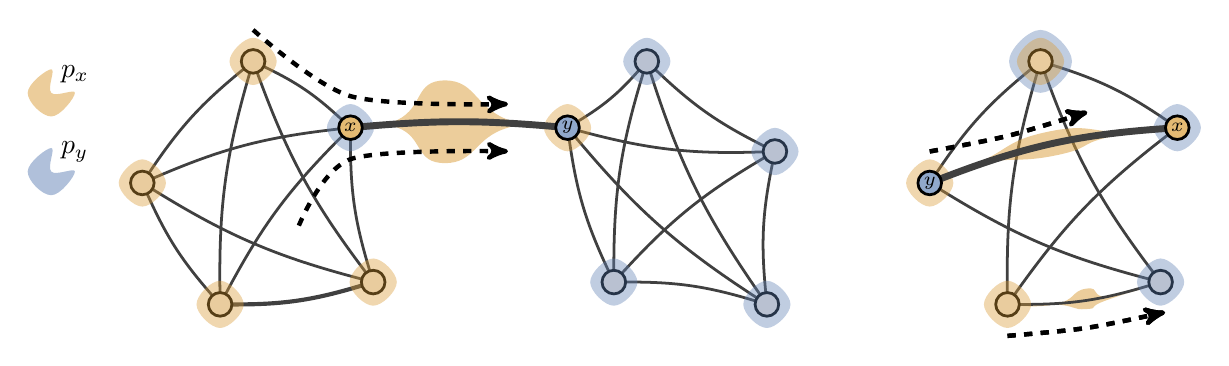
\begin{tikzpicture}[>=stealth']
    \Vertex[x=4.800,y=3.058,size=0.3,label=$x$,color=orange!70]{1}
    \Vertex[color=brokenwhite!30,x=3.563,y=3.900,size=0.3,label=]{2}
    \Vertex[color=brokenwhite!30,x=2.156,y=2.356,size=0.3,label=]{3}
    \Vertex[color=brokenwhite!30,x=3.144,y=0.814,size=0.3,label=]{4}
    \Vertex[color=brokenwhite!30,x=5.088,y=1.097,size=0.3,label=]{5}
    \Edge[lw=1,,bend=-8.531](1)(2)
    \Edge[lw=1,,bend=-8.531](1)(3)
    \Edge[lw=1,,bend=-8.531](1)(4)
    \Edge[lw=1,,bend=-8.531](1)(5)
    \Edge[lw=1,,bend=-8.531](2)(3)
    \Edge[lw=1,,bend=-8.531](2)(4)
    \Edge[lw=1,,bend=-8.531](2)(5)
    \Edge[lw=1,,bend=-8.531](3)(4)
    \Edge[lw=1,,bend=-8.531](3)(5)
    \Edge[,bend=-8.531](4)(5)

    \Vertex[x=7.556,y=3.058,size=0.3,label=$y$,color=blue!70]{11}
    \Vertex[color=brokenwhite!30,x=8.563,y=3.900,size=0.3,label=]{12}
    \Vertex[color=brokenwhite!30,x=10.190,y=2.756,size=0.3,label=]{13}
    \Vertex[color=brokenwhite!30,x=10.088,y=0.814,size=0.3,label=]{14}
    \Vertex[color=brokenwhite!30,x=8.144,y=1.097,size=0.3,label=]{15}
    \Edge[lw=1,bend=-8.531](11)(12)
    \Edge[lw=1,bend=-8.531](11)(13)
    \Edge[lw=1,bend=-8.531](11)(14)
    \Edge[lw=1,bend=-8.531](11)(15)
    \Edge[lw=1,bend=-8.531](12)(13)
    \Edge[lw=1,bend=-8.531](12)(14)
    \Edge[lw=1,bend=-8.531](12)(15)
    \Edge[lw=1,bend=-8.531](13)(14)
    \Edge[lw=1,bend=-8.531](13)(15)
    \Edge[lw=1,bend=-8.531](14)(15)

    \coordinate (label_x) at (1,3.5);
    \node[above right] (x) at (label_x) {$p_x$};
    \fill [orange, opacity=0.5] plot [smooth cycle, tension=0.7] coordinates {($ (label_x) + (0.3,0)$) ($ (label_x) + (0,-0.3)$) ($ (label_x) + (-0.3, 0)$) ($ (label_x) + (0,0.3)$) (label_x)};

    \coordinate (label_y) at (1,2.5);
    \node[above right] (y) at (label_y) {$p_y$};
    \fill [blue, opacity=0.5] plot [smooth cycle, tension=0.7] coordinates {($ (label_y) + (0.3,0)$) ($ (label_y) + (0,-0.3)$) ($ (label_y) + (-0.3, 0)$) ($ (label_y) + (0,0.3)$) (label_y)};


    \fill [orange, opacity=0.4] plot [smooth cycle, tension=0.7] coordinates {($ (2) + (0.3,0)$) ($ (2) + (0,-0.3)$) ($ (2) + (-0.3, 0)$) ($ (2) + (0,0.3)$)};
    \fill [orange, opacity=0.4] plot [smooth cycle, tension=0.7] coordinates {($ (3) + (0.3,0)$) ($ (3) + (0,-0.3)$) ($ (3) + (-0.3, 0)$) ($ (3) + (0,0.3)$)};
    \fill [orange, opacity=0.4] plot [smooth cycle, tension=0.7] coordinates {($ (4) + (0.3,0)$) ($ (4) + (0,-0.3)$) ($ (4) + (-0.3, 0)$) ($ (4) + (0,0.3)$)};
    \fill [orange, opacity=0.4] plot [smooth cycle, tension=0.7] coordinates {($ (5) + (0.3,0)$) ($ (5) + (0,-0.3)$) ($ (5) + (-0.3, 0)$) ($ (5) + (0,0.3)$)};

    \fill [blue, opacity=0.4] plot [smooth cycle, tension=0.7] coordinates {($ (12) + (0.3,0)$) ($ (12) + (0,-0.3)$) ($ (12) + (-0.3, 0)$) ($ (12) + (0,0.3)$)};
    \fill [blue, opacity=0.4] plot [smooth cycle, tension=0.7] coordinates {($ (13) + (0.3,0)$) ($ (13) + (0,-0.3)$) ($ (13) + (-0.3, 0)$) ($ (13) + (0,0.3)$)};
    \fill [blue, opacity=0.4] plot [smooth cycle, tension=0.7] coordinates {($ (14) + (0.3,0)$) ($ (14) + (0,-0.3)$) ($ (14) + (-0.3, 0)$) ($ (14) + (0,0.3)$)};
    \fill [blue, opacity=0.4] plot [smooth cycle, tension=0.7] coordinates {($ (15) + (0.3,0)$) ($ (15) + (0,-0.3)$) ($ (15) + (-0.3, 0)$) ($ (15) + (0,0.3)$)};

    \begin{scope}[on background layer]

        \fill [orange, opacity=0.4] plot [smooth cycle, tension=0.7] coordinates {($ (11) + (0.3,0)$) ($ (11) + (0,-0.3)$) ($ (11) + (-0.3, 0)$) ($ (11) + (0,0.3)$)};
        \fill [blue, opacity=0.4] plot [smooth cycle, tension=0.7] coordinates {($ (1) + (0.3,0)$) ($ (1) + (0,-0.3)$) ($ (1) + (-0.3, 0)$) ($ (1) + (0,0.3)$)};
        
        \fill [orange, opacity = 0.5] plot [smooth cycle, tension=1] coordinates {(1) ($ (1) + (0.6,0.1)$) ($ (1) + (1.2,0.6)$) ($ (1) + (2, 0.1)$) (11) ($ (1) + (2, 0)$) ($ (1) + (1.2,-0.45)$) ($ (1) + (0.6, 0)$)};
    \end{scope}

    \Edge[lw=2.5,bend=5](1)(11)

    \draw[ultra thick, dashed,->] plot[smooth] coordinates {($(2) + (0,0.4)$) ($(1) + (0,0.4)$) ($ (1) + (2, 0.3)$)};
    \draw[ultra thick, dashed,->] plot[smooth] coordinates {($(4) + (1,1)$) ($(1) - (0,0.4)$) ($ (1) + (2, -0.3)$)};

    \Vertex[x=15.300,y=3.058,size=0.3,label=$x$,color=orange!70]{21}
    \Vertex[color=brokenwhite!30,x=13.563,y=3.900,size=0.3]{22}
    \Vertex[color=blue!70,x=12.156,y=2.356,size=0.3,label=$y$]{23}
    \Vertex[color=brokenwhite!30,x=13.144,y=0.814,size=0.3]{24}
    \Vertex[color=brokenwhite!30,x=15.088,y=1.097,size=0.3]{25}
    \Edge[lw=1,,bend=-8.531](21)(22)
    \Edge[lw=1,,bend=-8.531](21)(24)
    \Edge[lw=1,,bend=-8.531](22)(23)
    \Edge[lw=1,,bend=-8.531](22)(24)
    \Edge[lw=1,,bend=-8.531](22)(25)
    \Edge[lw=1,,bend=-8.531](23)(25)


    \fill [orange, opacity=0.4] plot [smooth cycle, tension=0.7] coordinates {($ (22) + (0.3,0)$) ($ (22) + (0,-0.3)$) ($ (22) + (-0.3, 0)$) ($ (22) + (0,0.3)$)};
    \fill [orange, opacity=0.4] plot [smooth cycle, tension=0.7] coordinates {($ (24) + (0.3,0)$) ($ (24) + (0,-0.3)$) ($ (24) + (-0.3, 0)$) ($ (24) + (0,0.3)$)};
    \fill [blue, opacity=0.4] plot [smooth cycle, tension=0.7] coordinates {($ (25) + (0.3,0)$) ($ (25) + (0,-0.3)$) ($ (25) + (-0.3, 0)$) ($ (25) + (0,0.3)$)};



    \begin{scope}[on background layer]
        \fill [blue, opacity=0.4] plot [smooth cycle, tension=0.7] coordinates {($ (22) + (0.4,0)$) ($ (22) + (0,-0.4)$) ($ (22) + (-0.4, 0)$) ($ (22) + (0,0.4)$)};
            
        \fill [orange, opacity=0.4] plot [smooth cycle, tension=0.7] coordinates {($ (23) + (0.3,0)$) ($ (23) + (0,-0.3)$) ($ (23) + (-0.3, 0)$) ($ (23) + (0,0.3)$)};
        \fill [blue, opacity=0.4] plot [smooth cycle, tension=0.7] coordinates {($ (21) + (0.3,0)$) ($ (21) + (0,-0.3)$) ($ (21) + (-0.3, 0)$) ($ (21) + (0,0.3)$)};

        \fill [orange, opacity = 0.5] plot [smooth cycle, tension=1] coordinates {(23) ($ (23) + (0.6,0.25)$) ($ (23) + (1.5,0.65)$) ($ (23) + (2.5, 0.65)$) (21) ($ (23) + (2.3, 0.59)$) ($ (23) + (1.6,0.35)$) ($ (23) + (0.6, 0.24)$)};

        \fill [orange, opacity = 0.5] plot [smooth cycle, tension=1] coordinates {(24) ($ (24) + (0.6,0.)$) ($ (24) + (1.,0.2)$) ($ (24) + (1.3,0.1)$) (25) ($ (24) + (1.25,0.05)$) ($ (24) + (1,-0.06)$) ($ (24) + (0.6, 0)$)};

    \end{scope}

    \Edge[lw=2.5,,bend=-8.531](21)(23)
    \Edge[lw=1,,bend=-8.531](24)(25)

    \draw[ultra thick, dashed,->] plot[smooth] coordinates {($(23) + (0,0.4)$) ($(23) + (1,0.6)$) ($ (23) + (2, 0.9)$)};

    \draw[ultra thick, dashed,->] plot[smooth] coordinates {($(23) + (0,0.4)$) ($(23) + (1,0.6)$) ($ (23) + (2, 0.9)$)};
    \draw[ultra thick, dashed,->] plot[smooth] coordinates {($(24) + (0,-0.4)$) ($(24) + (1,-0.3)$) ($ (24) + (2,-0.1)$)};

    \draw[ultra thick, dashed,->] plot[smooth] coordinates {($(24) + (0,-0.4)$) ($(24) + (1,-0.3)$) ($ (24) + (2,-0.1)$)};
\end{tikzpicture}
\end{document}
